\documentclass[10pt,draftclsnofoot,onecolumn]{article}

\usepackage[letterpaper, total={7in, 9.5in}]{geometry}
\usepackage[utf8]{inputenc}
\usepackage{times} 
\usepackage[T1]{fontenc}         
\usepackage{pslatex}
\usepackage{bibentry}
\usepackage{graphicx}
\usepackage{listings}
\usepackage{color}
\usepackage{parcolumns}

%thanks to https://gist.github.com/FelipeCortez/10729134
\definecolor{bluekeywords}{rgb}{0.13, 0.13, 1}
\definecolor{greencomments}{rgb}{0, 0.5, 0}
\definecolor{redstrings}{rgb}{0.9, 0, 0}
\definecolor{graynumbers}{rgb}{0.5, 0.5, 0.5}

\bibliographystyle{plain}

\title{Operating Systems II Final Research Paper}

\author{Nicholas Milford}

\date{\today}

\begin{document}
\maketitle

\thispagestyle{empty}

\section{Introduction}

Linux, FreeBSD, and Windows are by far the most common operating systems for end-user devices. Comparing the internals of these operating systems leads to both a better understanding of each individually and where one might serve better than another. In this paper, three large components of each operating system will be analyzed and compared: the IO implementation, process management, and memory management. Advantages of each operating system will be discussed and concluded upon for each of the components.

\section{IO Comparison}

\subsection{High-Level Structure}

The basic architecture of the IO systems in all three operating systems is the same: provide an abstraction for all devices through a common open/close/read/write interface. In all three, that interface is the file system: File Descriptors in FreeBSD, Virtual Files in Windows, and the Common File Model in Linux \cite{Loonix,BSDM,Wandos}. It then becomes the responsibility of the driver to implement those commands and interface with the device directly. 
\\\\
In Windows, IO management within the system is achieved through use of IO Request Packets (IRPs). When an IO API function is called within a program, several steps are taken for that call to be fulfilled \cite{Wandos}:\\

\begin{enumerate}
	\item The IO manager creates the IO Request Packet, containing the API call, the file object, the device object, and the driver object
	\item The IO manager passes a pointer to the IRP to the appropriate driver
	\item The driver satisfies the IO operation, preparing an interrupt for when the task is completed
	\item When the interrupt fires, the driver handles it by notifying the IO manager that the task has been completed
	\item The IO manager completes the request and deletes the IRP
\end{enumerate}

\noindent The Windows IO manager’s packet-based system may seem to add unnecessary complexity and overhead, but it is necessary considering Windows’ microkernel architecture. Because a driver cannot directly communicate with another driver, it must communicate through the IO system. The packet system also allows for easier interoperability and flexibility between drivers, as will be seen when layered drivers are discussed. 
\\\\
The Linux and BSD kernels are much less complicated because the kernel is monolithic, meaning interaction between kernel modules is simpler. When a read or write call is made to a device file, the kernel calls the respective driver function, which then returns back up the call stack to the calling program after the hardware interaction has been completed \cite{BSDM,Loonix}. 
\\\\
Comparing these IO systems at this level does not yield much useful information to the end user. Both systems are built around the same user-space interface, meaning they only differ in implementation. From there, it is easy to see that the Windows system is much more complex and therefore likely has higher performance overhead than the more straightforward linux implementation. This is an incomplete explanation though, as that additional complexity comes from further design decisions made in regards to other aspects of the Windows IO system.

\subsection{Drivers}

Software that interacts with peripherals are implemented very differently in FreeBSD/Linux and Windows, mostly because of the monolithic kernel and microkernel design choice. Normally, under a monolithic kernel all device drivers are to be included at compile time and share the global kernel memory space. In practice, a module system has been developed to circumvent the driver inclusion limitation and allow drivers to be added to the monolithic kernel dynamically. The microkernel design pattern instead treats everything not essential to the minimal operation of the computer as a separate program. From the driver developer perspective, the most interesting difference that stems from the monolithic/microkernel divide is the Windows layered driver model.
\\\\
The Windows layered driver model is an extension of the flat model used in Linux and FreeBSD. It allows for intermediate drivers that can instead communicate with another driver above or below them, rather than only with the operating system and the device \cite{Wandos}. This model adds some complexity on the kernel end, but there are cases where additional layers of abstraction can improve the development process of drivers in some cases. Most of the time, more than one driver is involved in the operation of a device. Figure 1 illustrates such a case. Linux drivers, on the other hand, are self-contained routines. While they may make extensive use of kernel libraries, only one driver operates on a device at any time. \\

\begin{figure}[h!]
	\centering
	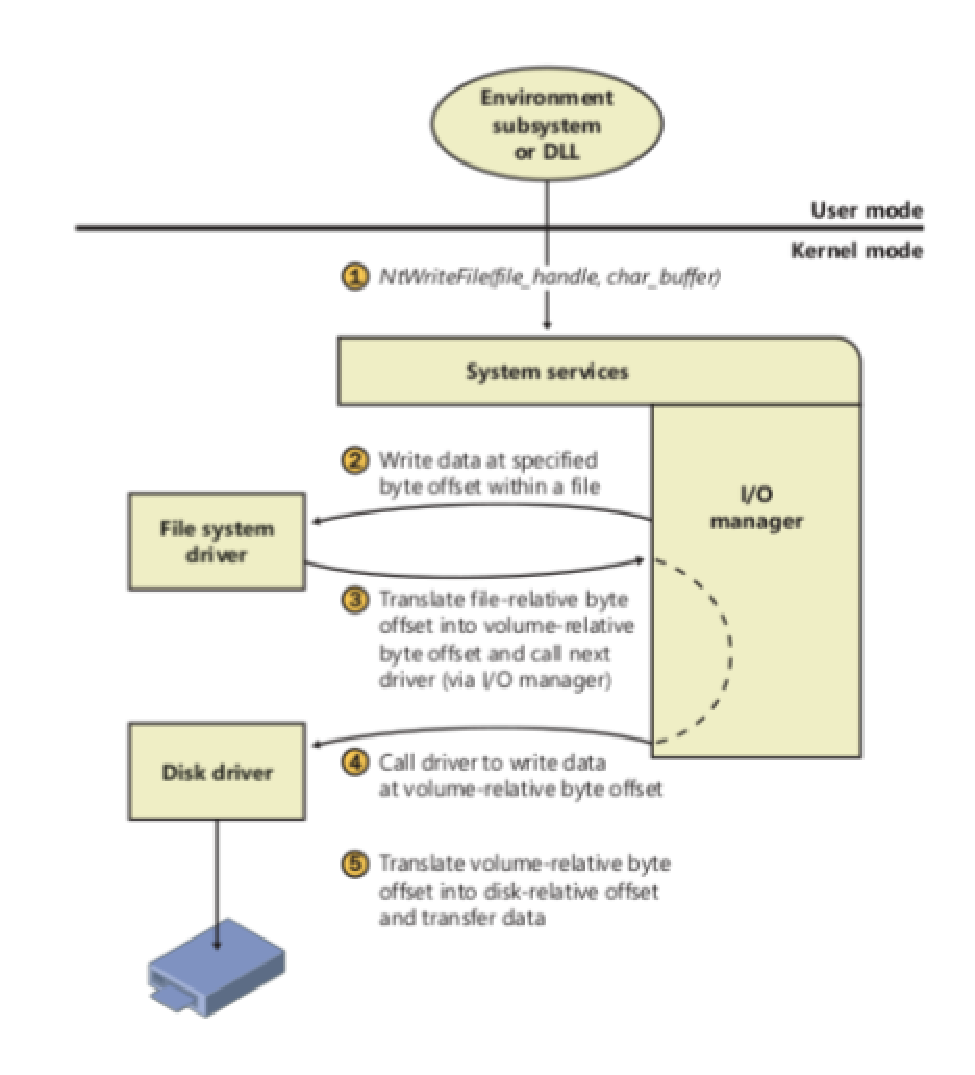
\includegraphics[width=3in]{wld}
	\caption{Diagram of a file system driver with two layers}
	\label{fig:layered}
\end{figure}

\noindent Inter-driver operation in Windows poses interesting conditions for a driver developer. In the case of a driver for a new variant on an existing class of devices, some of the drivers in the stack may be able to be reused. If the driver is for an entirely new device, then the rigid Windows framework would be more of a hindrance than a benefit, and so it would be easier to develop in Linux.

\subsection{Block/Character Devices}

Peripherals come in two rough categories: block and character. Character devices output a stream of bytes which are then interpreted by a driver. Block devices communicate by using entire blocks of characters at a time. Only the Linux IO system distinguishes between block and character devices for the purpose of driver development, with that distinction being implemented below the virtual file system.
\\\\
In FreeBSD, block devices are exposed in the same manner as character devices. Because of this, operations on block devices must be made in multiples of the device’s block size to work properly. FreeBSD does implement disk device drivers, which are character drivers extended with a strategy routine that handles block-like kernel-level calls \cite{BSDM}.
\\\\
There exists no clear information about the distinction between block and character devices in Windows. Instead, drivers are split into categories of filter drivers, function drivers, and bus drivers. \\

\begin{itemize}
	\item Filter drivers “augment or change the behavior of a device or another driver” \cite{Wandos}. 
	\item Bus drivers manage a bus-style device or internal structure, and so lies closest to the hardware.
	\item Function drivers expose the device interface to the IO manager, and by extension the operating system. Normally, this driver manages the operation of the device.
\end{itemize}

\noindent In the layered driver model, bus drivers lie at the bottom, managing computer specific hardware. Function and Filter drivers may be interspersed above the bus driver in any order. 

\subsection{IO Management Conclusion}

The choice of one IO system implementation over another based on the differences discussed here only really has implications towards the driver developers. Generally, driver development would be easiest on Linux or FreeBSD, though there are some specific cases where Windows would be the easier to develop on. This lines up with the biggest use-case divide between Windows and Linux: Windows dominates the desktop market, while Linux is used almost exclusively in operating systems for embedded systems.

\section{Process Management Comparison}

\subsection{Process Creation}

Process creation is implemented completely differently in Windows and FreeBSD/Linux. Both FreeBSD and Linux use the fork and exec model, where a process descriptor is mostly copied within the operating system and continues running after the fork instruction. Process ID, parent process ID, and some resources are not copied. The Linux implementation does not copy the program’s working space immediately, instead utilizing copy-on-write (COW) to only copy parts of memory that are written to by the child or parent process. After forking, an exec call is usually used to replace the current program with a new one and the process is started from the beginning \cite{Wandos}. This is illustrated in listing 2.
\\\\
In Windows, when a CreateProcess() function is called, the parent process first creates a new thread object from a given executable file, containing the entire process context. This involves creating memory space for the thread, setting up kernel-level data structures, and inheriting necessary flags and fields from the parent. The thread object is then handed to the Windows subsystem, which initializes all fields necessary to scheduling and management at the kernel level. Finally, the process is added to the system-wide process queue and is ready to be run \cite{Wandos}. An example of this usage can be found in listing 1.\\

\lstset{language=C,
	basicstyle=\ttfamily,
	keywordstyle=\color{bluekeywords}\ttfamily,
	stringstyle=\color{redstrings}\ttfamily,
	commentstyle=\color{greencomments}\ttfamily
}

\noindent\begin{minipage}{.48\textwidth}
	\begin{lstlisting}[caption=Creating a new process in Windows in user space~\cite{creating-processes},frame=tlrb]{Name}
STARTUPINFO si;
PROCESS_INFORMATION pi;

ZeroMemory( &si, sizeof(si) );
si.cb = sizeof(si);
ZeroMemory( &pi, sizeof(pi) );

// Start the child process. 
if( !CreateProcess( NULL,   //module name
    argv[1],        //Command line
    NULL,           //Process handle 
    NULL,           //Thread handle
    FALSE,          //Handle inheritance
    0,              //Creation flags
    NULL,           //Environment block
    NULL,           //Starting directory 
    &si,            //STARTUPINFO
    &pi )           //PROCESS_INFORMATION
) 
{
    printf("CreateProcess failed");
    return;
}
	\end{lstlisting}
\end{minipage}\hfill
\begin{minipage}{.45\textwidth}
	\begin{lstlisting}[caption=Creating a new process in Linux/BSD in user space,frame=tlrb]{Name}
if(pid = fork()){ //parent
	...
}
else{ // child
	...
	//exec
	execvp(args[0], args);
}
	\end{lstlisting}
\end{minipage}

\subsection{Process Scheduling}

High level process scheduling works similarly in the Windows scheduler and Linux’s CFS. Both use one small process queue per CPU that pull from a system-wide collection of threads or processes. This system-wide collection consists of one queue for each possible priority level, 32 for Windows and 140 for Linux \cite{Wandos}. Priority levels are divided up into real-time and variable intervals as described in table 1.\\

\begin{table}
	\centering
		\begin{tabular}{ | l | c | r | }
			\hline
			& Real-Time Levels & Normal Levels \\\\ \hline
			Linux/FreeBSD & 0 - 99 & 100 - 139 \\\\ \hline
			Windows & 16 - 31 & 1 - 15 \\\\ \hline
		\end{tabular}
		\caption{designated real-time and normal priority levels}
	\centering
\end{table}

\noindent The ULE scheduler implemented in FreeBSD uses three queues per CPU: two for running processes and one for the idle process. The two running process queues are labeled as “current” and “next”. The CPU takes processes from the “current” queue and runs them for their respective time slot until all processes in the queue have been run, after which the “current” queue is switched with the “next” queue. Real-Time threads, low-latency or interactive processes, and interrupts are placed directly into the “current” queue when scheduled, while all other processes are placed in the “next” queue \cite{Roberson03ule:a}. 
\\\\
The ULE scheduler avoids CPU time starvation by guaranteeing every scheduled thread is run once every two queue switches, however the only way to guarantee a low-latency thread is run often is by preempting another thread \cite{Roberson03ule:a}. The Windows and Linux scheduling implementations can guarantee a minimum start time because CPU queues are kept minimal, instead storing process identifiers in one system-wide structure. The drawback of this is that complete resource starvation of medium priority threads during high utilization is only prevented through the implementation of thread priorities and run times.

\subsubsection{Process Prioritization}

FreeBSD and Linux use the same thread prioritization methodology of determining interactivity of a thread for a first rough categorization, and then refining priority through a process’s “nice” value. Interactivity is a simple ratio of how much time the process spent sleeping and how much time was spent running over the last five seconds (see figure 3). If a thread’s interactivity passes a threshold, it is labeled as “interactive” and will be run more often, but for smaller amounts of time. “Nice” values are set at execution time and determine the proportion of CPU time the process gets during each time slice. A lower “nice” value means the process will use more CPU time \cite{215951, Roberson03ule:a}. 
\\\\	
The Windows scheduler also uses two priority classifications to determine the full priority level of a process: a process’s priority class, and a thread’s relative priority. Priority classes of processes are set through the Windows API. Usually this is during the process creation, but it can be changed by the user. Relative priority is adjusted throughout runtime and adjusts the priority of the thread from the process base priority. Priority will only be adjusted by 1 or 2 levels unless the thread is deemed “time critical” or “idle”. Relative priority can not give a non-real-time thread a real-time priority, and vice versa \cite{Wandos}. 
\\\\
Comparatively, the FreeBSD and Linux prioritization schemes allow for more granular control by the user with “nice” values that can take on any value from -20 to 19, as opposed to the Windows prioritizer, which only has categories of “realtime”, “high”, “above normal”, “normal”, “below normal”, “low”, and “idle”. The Windows prioritizer maintains finer control of thread priorities, as a thread in FreeBSD or Linux is only “interactive” or “not interactive”. Thus the two implementations may have advantages in different scenarios.

\subsubsection{Process Run Times}

How long a process is run for at one time again differs by operating system. Windows will run a process for one quantum at a time, which is a system-wide value of 2 clock intervals for client systems and 12 clock intervals on servers. Processes may run for less than one quantum if preempted by a higher priority process, and may run for multiple quantums if there are no processes of the same priority level waiting to run \cite{Wandos}.
\\\\
Linux and FreeBSD dynamically vary the quantum length of each process according to the “nice” value of the process. Lower “nice” values are given larger proportions of a time slice than processes with higher “nice” values. In Linux’s CFS, if there are more processes than there are minimum sized quanta to go around, then the time slice increases in size, and so no process is completely starved for CPU resources. The ULE scheduler works slightly differently for large thread loads: processes that have a “nice” value more than 20 values away from the least “nice” process are not run at all. Then, if there are more processes than minimum sized quanta, the time slice length is increased \cite{Love:2005:LKD:1214858, Roberson03ule:a}.
\\\\
The fixed-time quanta and variable quanta methods used by Windows and CFS/ULE are hard to compare without extensive test data, because each has a different type of overhead: fixed-time quanta has the overhead of rescheduling threads after every quanta even if there are no other threads of the same priority to run, while the variable quanta method does more calculations in setting up time slices in order to avoid frequent micromanagement. The other difference of note is that Windows and ULE allow for thread starvation, though Windows allows it as an incident of how the scheduler was designed while the feature was deliberately build into ULE. Linux’s Completely Fair Scheduler, true to its name, does not allow for a thread to be completely CPU time starved, regardless of priority. 

\subsection{Process Management Conclusion}

The choice of one operating system over another for process management purposes depends heavily on use case requirements, because the advantages of one operating system over another vary in significance and best choice. For embedded systems, it may be necessary that all processes be run all the time, in which case Linux’s completely fair scheduler would be the best choice. If reaction to interrupts and other time-sensitive events are a high priority, then FreeBSD’s ULE scheduler is out of the question. If fixed-time process run times would be an advantage, then Windows will be the best option. For the desktop user though, the ULE scheduler seems to be the best option: its finer control over process and thread priorities allows for better performance tuning, and the ability for it to not run the lowest priority threads is an advantage for a human only looking at one process at a time.

\section{Memory Management Comparison}

\subsection{Address Translation}

When working in the virtual address space of a process, subsections of memory may be dynamically allocated or temporarily removed by the operating system. Thus the translation from a virtual address to a physical address in RAM becomes nontrivial. The implementation of address translation has converged in all of Windows, FreeBSD, and Linux: All implement a two-level page table that uses a 32-bit virtual address. The first 10 bits are used to index the first table, and the second 10 bits are used to find the first table that is indexed by the value of the first table. The last 12 bits of the virtual address, the byte offset, is then applied to get the exact byte within the page \cite{BSDM, Wandos, Loonix}.
\\\\
This convergence is due to the adoption of hardware-implemented address translation in the MMU. As dedicated hardware solutions will be faster than any software running in the kernel on the general-purpose CPU, software implementations of virtual memory address translation were deprecated in modern operating systems.

\subsection{Page Caching}

When a virtual address is translated and its page retrieved, it is placed into a page cache in memory, allowing faster subsequent reads. Because the space in the page cache is limited, and the speed increase significant, memory management systems must decide which pages to cache and which to remove from the cache when more space is needed. 
\\\\
The structure of the page cache varies slightly between FreeBSD, Linux, and Windows. FreeBSD and Linux use page lists: FreeBSD uses three lists, one for “free” pages which voluntarily go there when a process exits, one for “inactive” pages, and one for “cache” or more active pages \cite{BSDM}. Linux only uses “active” and “inactive” lists, one each \cite{Loonix}. No information could be found on the data structure used in Windows to manage the page cache.
\\\\
Two sub-features of the page caching system have the most impact in the performance of the caching algorithm (usually measured in fault rate, or the ratio of page faults to pages accessed) \cite{BSDM}. These are the fetch and replacement policies, or when to add pages to the cache and which pages to remove to make space for new pages. Many algorithms for both problems have been designed for page caches in particular. 

\subsubsection{Page Replacement}

Linux uses a simplified least-recently-used algorithm, where pages are given “in use” or “unused” labels \cite{Loonix}. Windows and FreeBSD use least-actively-used policies, but with slight variations \cite{BSDM, Wandos}. Both aim to find the pages that are least likely to be used in the near future.
\\\\
The page replacement algorithm employed by Linux requires only two flags per page and the “active” and “inactive” lists mentioned earlier. When a page is accessed, the “referenced” bit is set. If the page is accessed again before the bit is cleared, then it is moved to the “active” list if it is not already in the “active” list, and the “active” bit is set for the page. When the memory manager scans the page, the “referenced” bit is cleared. Pages are moved from the “active” list to the “inactive” list when the memory manager periodically rebalances the lists, or when the system is low on memory. Only pages in the “inactive” list may be paged out to make space for new pages [3]. A much more concise explanation is provided in figure 1.\\

\begin{figure}[h!]
	\centering
	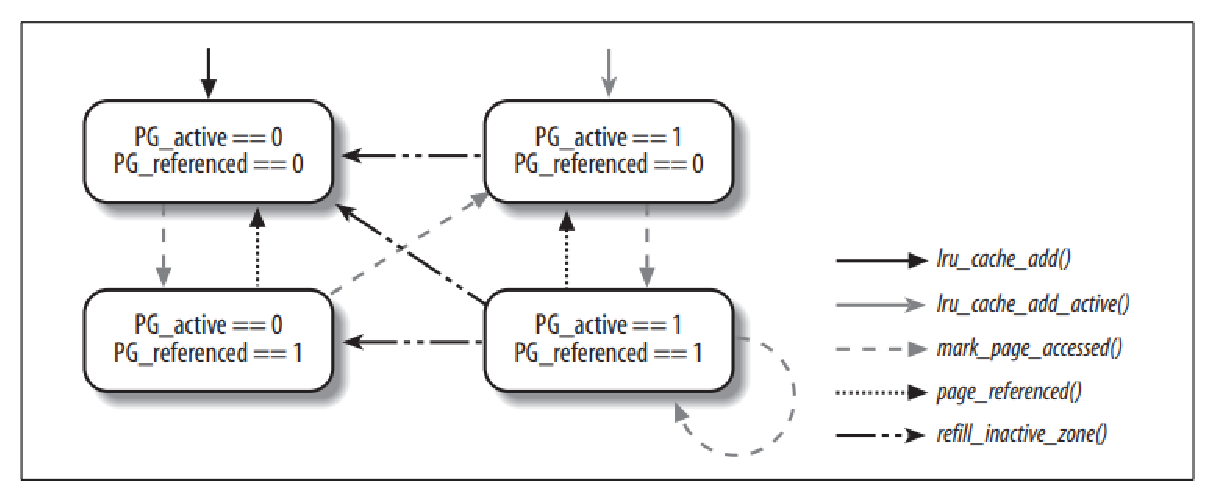
\includegraphics[width=3in]{linuxPagingAlg}
	\caption{Diagram of a file system driver with two layers}
	\label{fig:layered}
\end{figure}

\noindent The least-actively-used policies in FreeBSD and Windows aim for finer granularity of page activity and therefore more accurate page swapping. Every page starts with an “age” in Windows and a “usage count” in FreeBSD. When a page is scanned by the memory manager and has not been accessed recently, its “age” is incremented or its “usage count” is decremented. In FreeBSD, if a page has been accessed recently then its “usage count” is incremented; in Windows, a page’s “age” cannot be decremented. Pages with a “usage count” of zero are moved to an “inactive” list and can be paged out, while pages with the highest “age” are the first to go in Windows \cite{Wandos, BSDM}.
\\\\
Of the three implementations, FreeBSD seems to be the superior. The oversimplicity of the Linux implementation leave it overly susceptible to short, infrequent periods of high memory activity by background processes. The Windows age implementation would be equivalent if not for the limitation that age never decreases, which causes the algorithm to eventually page out pages that are used periodically, only for them to be re-fetched when needed again.

\subsubsection{Page Fetching}

The implementations of the page fetch policy for the three operating systems vary less drastically than those of the page replacement policy, though still have unique solutions. Linux uses the simplest possible solution of pure demand-paging: only the page requested is loaded into the cache upon a page fault. 
\\\\
Windows and FreeBSD seek better performance by loading more pages than just the requested one, or “prepaging”. They expect that a need for these extra pages logically follows from the need of the first page. This feature is called “page clustering” by both operating systems. Windows loads an additional 2 or 6 pages around the requested page, where no exact information could be found about how FreeBSD clusters pages on fetch \cite{Wandos, BSDM}.
\\\\
Windows has an additional feature called the “logical prefetcher”. This has one purpose: to speed up the startup time of the system and large applications by learning which pages in memory are used soon after startup, eliminating the need to wait for a page fault for those particular pages \cite{Wandos}.
\\\\
In the end, the outcome of the three different page fetch variations are similar to that of the page replacement algorithms: Linux implements the simplest solution, but in its simplicity loses performance and efficiency. FreeBSD and Windows use more complex but similar designs, but this time it is the extra features of Windows that make it seem like the best candidate. 

\subsection{Memory Management Conclusion}

All three operating systems were built with the same memory management design goals in mind. For address translation, these common design goals manifested in a single hardware solution that is now universally adopted. In page fetching and replacement, different approaches were made to trade off simplicity for performance, or additional side-features were added to further extend performance.

\section {Conclusion}

For the lower-level developer, the choice is clear: FreeBSD or Linux provide the easiest to use interfaces for creating and managing processes and IO. These systems will also likely be easier to develop new drivers for. Real-time or memory requirements will further determine if FreeBSD or Linux is the better choice for this case. For the user, more concerned about reactivity and performance, FreeBSD’s memory management and process scheduling systems give it the advantage. Further use cases will have different best options, and it is impossible to enumerate them all here, especially considering that no one operating system can be universally said to be the best at any of the components discussed.

\clearpage
\bibliography{final}

\end{document}

